
\tikzstyle{process} = [rectangle, fill=blue!20, minimum width=2.5cm, minimum height=1cm, text centered, draw=black]
\tikzstyle{arrow} = [thick,->,>=stealth]

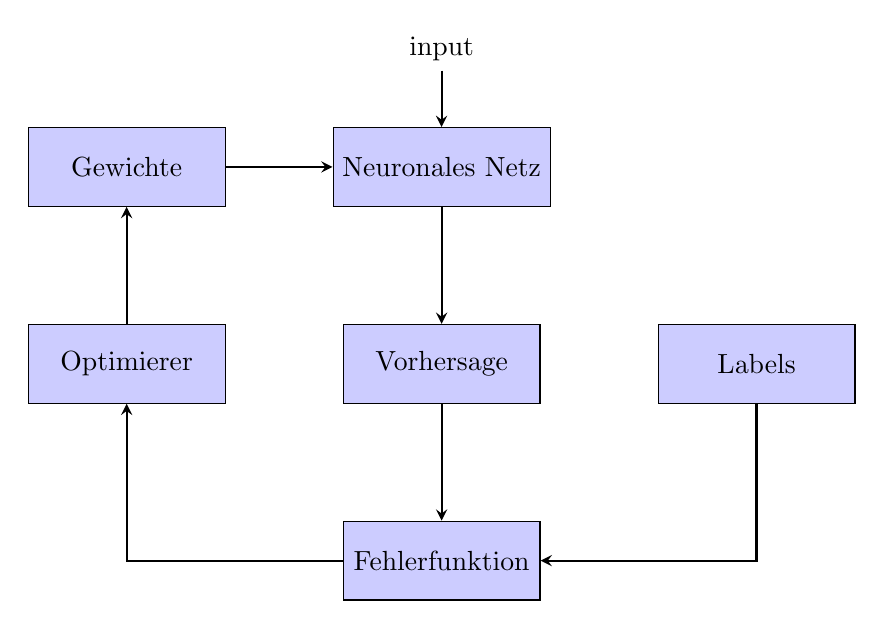
\begin{tikzpicture}[node distance=1.6cm]

  \begin{scope}[node distance=2.5cm]
    \node (nn)      [process]                   {Neuronales Netz};
    \node (pred)      [process, below of=nn]      {Vorhersage};
    \node (loss)      [process, below of=pred]      {Fehlerfunktion};
    
  \end{scope}
  
  \begin{scope}[node distance=4cm]
    \node (opt) [process, left of=pred]      {Optimierer};
    \node (weights)  [process, left of=nn] {Gewichte};
    \node (labels)   [process, right of=pred]  {Labels};
  \end{scope}

  \node (input) at (0,1.5) {input};

  \draw[arrow] (input) -- (nn);

  \draw[arrow] (nn) -- (pred);
  \draw[arrow] (pred) -- (loss);

  \draw[arrow] (labels) |- (loss);
  \draw[arrow] (loss) -| (opt);

  \draw[arrow] (opt) -- (weights);
  \draw[arrow] (weights) -- (nn);
  
    
\end{tikzpicture}
